\section*{CHAPTER 3: APPROACH}
\addcontentsline{toc}{section}{\numberline{}CHAPTER 3: APPROACH}
\label{sec:approach}
\setcounter{section}{3}
\setcounter{subsection}{0}
\setcounter{figure}{0}
\setcounter{table}{0}

\subsection{Architecture}
\label{sec:architecture}
 
The implementation is organised in layers, with dependencies pointing in one
direction only:
 
% \begin{verbatim}
%                     notebooks (01-05)                     presentation
%                            |
%    +---------+-------------+-------------+----------+
%    |         |             |             |          |
%   eda   preprocessing  classical     neural    embeddings        business
%    |         |         evaluation -- metrics    ensemble           logic
%    |         |          validity    error_analysis
%    +---------+-------------+-------------+----------+
%                            |
%                   +--------v--------+
%                   | IssueRepository |                     abstract interface
%                   +--------+--------+
%              +-------------+-------------+
%    InMemoryIssueRepository      FileIssueRepository        persistence
%            (RAM)                   (CSV / JSON)
% \end{verbatim}

\begin{figure}[htbp]
  \centering
  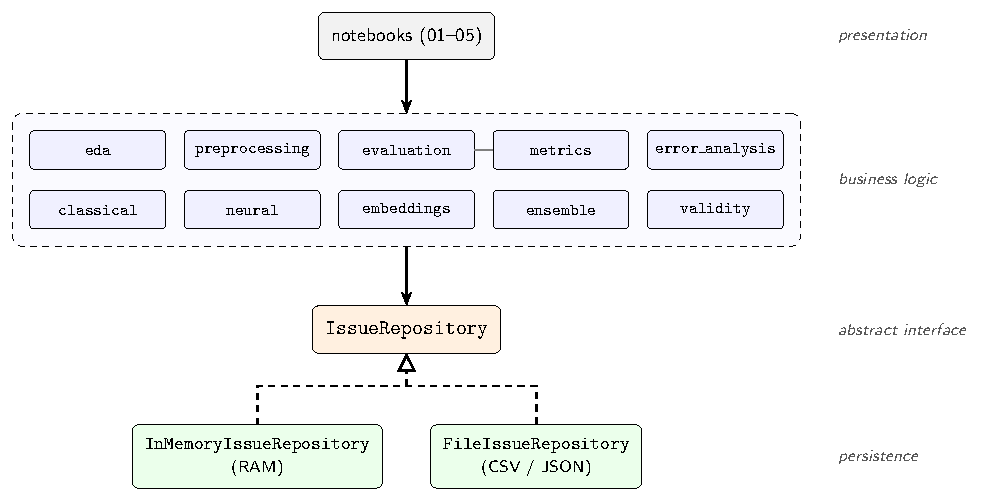
\includegraphics[width=\linewidth]{figures/architecture.pdf}
  \caption{Layered architecture. Solid arrows are dependencies; dashed arrows
           with open heads mark implementations of the abstract interface.}
  \label{fig:architecture}
\end{figure}
 
Persistence knows nothing about analysis, and analysis knows nothing about
storage. \texttt{IssueReport}, the single domain entity, depends on nothing.
 
The layering is also implemented by dependency weight. The domain, persistence,
preprocessing, metrics and evaluation layers require only pandas, matplotlib and
NLTK; \texttt{import ai4se} works with neither scikit-learn nor PyTorch installed, and
the model tracks are imported from submodules on demand. A test parses the
package source to keep it that way, so a team member unable to install PyTorch
is not blocked from any other part of the project.
 
\subsection{Persistence layer}
\label{sec:persistence}
 
The project specification requires that data be manageable both in memory and
through files, and that switching between the two involve few changes to the
application. We implement this with the Repository pattern.
 
\texttt{IssueRepository} is an abstract base class exposing \textbf{five primitives}
--- \texttt{load}, \texttt{save}, \texttt{all}, \texttt{add}, \texttt{clear} --- and
roughly a dozen query helpers (\texttt{by\_repo}, \texttt{by\_label},
\texttt{label\_distribution}, \texttt{texts\_and\_labels}, \texttt{filter},
\texttt{apply}, \texttt{to\_dataframe}, and the standard container protocol). The
helpers are implemented \textbf{once, on the base class}, in terms of the five
primitives.
 
This makes behavioural equivalence structural: adding a
query adds it to both implementations simultaneously, and they cannot drift apart. \texttt{InMemoryIssueRepository} wraps a Python list and its
\texttt{load}/\texttt{save} are deliberate no-ops; \texttt{FileIssueRepository}
reads and writes CSV or JSON, inferring the format from the file suffix.
 
Switching the entire application's persistence layer is one argument:
 
\begin{verbatim}
train = load_split("train", kind="memory")   # held in RAM
train = load_split("train", kind="file")     # backed by the CSV on disk
\end{verbatim}
 
\textbf{Evidence.} \texttt{tests/test\_persistence\_equivalence.py} runs the
identical analysis pipeline (load, clean, extract features and labels) over
both layers and asserts that the results match shown in Table~\ref{tab:persistence-equivalence}
 
% \begin{table}[H]
%   \centering
%   \begin{tabular}{@{}llll@{}}
%     \toprule
%     Property & In-memory & File & Equal \\
%     \midrule
%     \texttt{n}            & 1500                        & 1500                        & yes \\
%     \texttt{distribution} & bug 500, feature 500, question 500   & bug 500, feature 500, question 500   & yes \\
%     \texttt{checksum}     & 658455                      & 658455                      & yes \\
%     \texttt{first\_label} & \texttt{bug}                & \texttt{bug}                & yes \\
%     \midrule
%     \multicolumn{3}{@{}l}{All properties identical} & \textbf{yes} \\
%     \bottomrule
%   \end{tabular}
%   \caption{Output of \texttt{tests/test\_persistence\_equivalence.py}: the same
%            pipeline run over both persistence layers.}
%   \label{tab:persistence-equivalence}
% \end{table}

\begin{table}[H]
  \centering
  \begin{tabularx}{\linewidth}{@{} l X X c @{}}
    \toprule
    Property & In-memory & File & Equal \\
    \midrule
    \texttt{n}            & 1500 & 1500 & yes \\
    \texttt{distribution} & bug: 500, feature: 500, question: 500 
                          & bug: 500, feature: 500, question: 500 & yes \\
    \texttt{checksum}     & 658455 & 658455 & yes \\
    \texttt{first\_label} & \texttt{bug} & \texttt{bug} & yes \\
    \midrule
    \multicolumn{3}{@{}l}{All properties identical} & \textbf{yes} \\
    \bottomrule
  \end{tabularx}
  \caption{Output of \texttt{tests/test\_persistence\_equivalence.py}: the same pipeline run over both persistence layers.}
  \label{tab:persistence-equivalence}
\end{table}
 
The same test verifies that CSV and JSON round-trips are lossless and that both
implementations satisfy the full abstract interface. Every function in the EDA,
evaluation and validity modules takes an \texttt{IssueRepository}, so the entire
analysis runs unchanged against either.
 
One implementation detail: \texttt{csv.field\_size\_limit} must be raised at
import, because the 21,595-word issue in Section~2.3 exceeds Python's default
field limit.
 
\subsection{Preprocessing}
\label{sec:preprocessing}
 
Each cleaning step is a pure \texttt{str} $\rightarrow$ \texttt{str} function, so
the pipeline can be reordered or partially disabled for ablation. Three levels are
selectable by one string shown in Table~\ref{tab:preprocessing-levels}
 
\begin{table}[htbp]
  \centering
  \begin{tabular}{@{}l p{7.5cm} l@{}}
    \toprule
    Level & Operations & Intended consumer \\
    \midrule
    \texttt{raw}   & whitespace normalisation only & control condition \\
    \texttt{light} & strips fenced code, stack traces, Markdown markup, URLs,
                     file paths, commit hashes, issue references, mentions
                   & transformer models \\
    \texttt{full}  & \texttt{light} + lowercasing, punctuation removal, stop
                     words, lemmatisation
                   & TF-IDF models \\
    \bottomrule
  \end{tabular}
  \caption{Preprocessing levels.}
  \label{tab:preprocessing-levels}
\end{table}
 
Stop words are NLTK's English list plus a domain list of terms appearing in
nearly every issue regardless of class (\texttt{issue}, \texttt{reproduce},
\texttt{expected}, \texttt{screenshot}, and similar).
 
\textbf{The configuration selected by ablation} (Section~5.1) is
\texttt{level="light"}, with the title repeated three times and the text truncated
to 200 words. Titles are short and dense with class-characteristic vocabulary, so
repeating them up-weights them in a bag-of-words representation at no cost. We
emphasise that \texttt{full}, which is the default in most text-classification
pipelines, is \textbf{not} what we use, for reasons Section~5.1 reports.
 
\subsection{Models}
\label{sec:models}
 
All models expose the same \texttt{fit(X, y)} / \texttt{predict(X)} interface and
are supplied to the evaluation harness as zero-argument factories, so that each
cross-validation fold and each repository receives a fresh untrained instance.
Models that also expose \texttt{predict\_proba} additionally get ROC and AUC
reported.
 
\subsubsection{Reference floors}
\label{sec:reference-floors}
 
\textbf{Majority class}, \textbf{stratified random}, \textbf{keyword rules} over
cue words drawn from Section~2.5, and \textbf{multinomial naive Bayes} implemented
from scratch in log space with Laplace smoothing.
 
\subsubsection{Classical machine learning}
\label{sec:classical-ml}
 
Five scikit-learn pipelines over a shared TF-IDF representation, so that score
differences come from the classifier rather than the features: multinomial naive
Bayes, complement naive Bayes, logistic regression, linear SVM, and random
forest.
 
\textbf{Vectorisation happens inside each pipeline, and therefore inside each
cross-validation fold.} Fitting the vectoriser once over the whole dataset before
cross-validating would leak test-fold vocabulary and document frequencies into
training and inflate every reported score. We guard against this with a dedicated
test.
 
Selected settings after grid search: bigrams for both linear models; logistic
regression at \texttt{C=10, min\_df=2}; linear SVM at \texttt{C=1, min\_df=1}.
\texttt{LinearSVC} has no probability head, so its AUC is reported as absent
rather than approximated.
 
\subsubsection{Neural networks}
\label{sec:neural}
 
\textbf{Feed-forward network} over TF-IDF features (20,000 max features, hidden
layers of 256 and 64, ReLU, dropout 0.5) directly comparable with the
classical pipelines.
 
\textbf{1-D convolutional network} over learned 100-dimensional embeddings, with
parallel filters of widths 2, 3 and 4 acting as learned n-gram detectors, 64
filters each, and global max-pooling.
 
Both hold out 20\% of the training data for validation and record training loss,
validation loss and validation accuracy at every epoch, with early stopping after
8 epochs without improvement, restoring the weights from the best epoch.
 
\subsubsection{Sentence transformers}
\label{sec:sentence-transformers}
 
\textbf{Frozen encoder baselines.} A pretrained Sentence Transformer encodes each
issue and a logistic-regression head is fitted on the embeddings; the encoder is
not updated. We evaluate \texttt{all-MiniLM-L6-v2} (6 layers, 384 dimensions) and
\texttt{all-mpnet-base-v2} (12 layers, 768 dimensions). This configuration is
precisely \textbf{SetFit with the contrastive fine-tuning step removed}, which is
what makes the decomposition in Section~5.4 possible.
 
\textbf{SetFit reproduction.} Generate pairs from the labelled examples,
fine-tune the encoder contrastively, then fit a logistic-regression head on the
adapted embeddings: 20 pair-generation iterations, 1 epoch.
 
Contrastive training embeds both sentences of every pair, so MPNet at MiniLM's
settings exceeds 12\,GB of GPU memory. We therefore run MPNet at
\texttt{batch\_size=8, max\_seq\_length=128}, and critically also run
MiniLM at those same settings, so that the encoder comparison is controlled.
 
\subsubsection{Ensembles}
\label{sec:ensembles}
 
Soft voting over the averaged class probabilities of two or three members. Soft
rather than majority voting because with three classes and two members, hard
votes tie often, and the tie discards exactly the confidence information that
would resolve it. Members were chosen because they fail on different projects
(Section~5.5).
 
\subsection{Reproducibility infrastructure}
\label{sec:reproducibility}
 
A single entry point regenerates every number in this report:
 
\begin{verbatim}
python scripts/run_experiments.py --all
\end{verbatim}
 
Nine stages write JSON results to \texttt{results/tables/} and figures to
\texttt{results/figures/}. Each skips work already on disk unless forced. The
notebooks read those saved results rather than re-training, and the LaTeX tables
are generated from the same JSON, so the numbers here cannot drift from what the
code produced. A fixed seed of 42 is used throughout.
 